% !TEX TS-program = pdflatex
% !TEX encoding = UTF-8 Unicode


\documentclass[11pt, nofootinbib]{article} 

\usepackage[utf8]{inputenc} 
\usepackage[dvipsnames, table]{xcolor}


\usepackage{geometry} 
\geometry{a4paper} 

\usepackage{graphicx} % support the \includegraphics command and options
\usepackage{pgf-pie}  
\usepackage{csvsimple}
\usepackage{datatool}
\usepackage{makecell}
\usepackage[group-separator={,},group-minimum-digits=4]{siunitx}
\usepackage{eso-pic}



\usepackage{booktabs} % for much better looking tables
\usepackage{array} % for better arrays (eg matrices) in maths
\usepackage{paralist} % very flexible & customisable lists (eg. enumerate/itemize, etc.)
\usepackage{verbatim} % adds environment for commenting out blocks of text & for better verbatim
\usepackage{subfig} % make it possible to include more than one captioned figure/table in a single float
% These packages are all incorporated in the memoir class to one degree or another...

%%% HEADERS & FOOTERS
\usepackage{fancyhdr} % This should be set AFTER setting up the page geometry
\usepackage{hyperref}
\pagestyle{fancy} % options: empty , plain , fancy
\renewcommand{\headrulewidth}{0pt} % customise the layout...
\lhead{}\chead{}\rhead{}



\pagestyle{fancy}
\fancyhf{}
\fancyhead[L]{\leftmark}
\cfoot{\thepage}
\rfoot{
    \vspace*{1cm}
    \includegraphics[width=2cm, height=2cm]{jklimage.png}
    \hspace*{-2cm}
  }

%%% SECTION TITLE APPEARANCE
\usepackage{sectsty}
\allsectionsfont{\sffamily\mdseries\upshape} % (See the fntguide.pdf for font help)
% (This matches ConTeXt defaults)

%%% ToC (table of contents) APPEARANCE
\usepackage[nottoc,notlof,notlot]{tocbibind} % Put the bibliography in the ToC
\usepackage[titles,subfigure]{tocloft} % Alter the style of the Table of Contents
\renewcommand{\cftsecfont}{\rmfamily\mdseries\upshape}
\renewcommand{\cftsecpagefont}{\rmfamily\mdseries\upshape} % No bold!



%%% END Article customizations

%%% The "real" document content comes below...

\title{JACKAL Protocol Economic Paper}
\author{Jackal Labs}
%\date{} % Activate to display a given date or no date (if empty),
         % otherwise the current date is printed 


\begin{document}
\begin{titlepage}
    \centering
    \vspace*{3cm}
    \includegraphics[width=4cm]{jklimage.png} % also works with logo.pdf
    \vskip2cm
    {\bfseries\Large
        JACKAL Economic Paper\\
        \vskip0.5cm
    }    
   {\bfseries
        Jackal Labs\\
    }    
    \vfill
    v 2.0.0. \\
    Prepared for public release
\end{titlepage}
%\maketitle
\newpage
\tableofcontents
\newpage



\section{Tokenomics}

This document will detail the economic structure of Jackal. All amounts are expressed in \$JKL unless otherwise specified.
The \$JKL token is an inflationary token and has four main functions: to be used for governance, storage provider
incentivization, validator incentivization, and access to Jackal Protocol appliactions. 

\section{Governance}

Jackal Protocol is an L1 blockchain on the Cosmos IBC and subject to governance
by the holders of \$JKL. Proposals towards Jackal Protocol cost \$JKL. Governance
of the is consistent with all other IBC governance models otherwise.


\section{Storage Provider Incentivization}

Jackal Protocol is supported by Jackal Storage Providers that supply storage space and support file
retrieval. As this peer-to-peer network is paramount to the success of the Protocol it is vital to incentivize
storage provider to maintain the network. Storage providers are rewarded with \$JKL in return for storing data and participating in Jackal Proof of Persistence.
Of the total block rewards at genesis approximately 60\% is alloocated to storage providers.

\section{Applications}

Along with its flagship storage product, Jackal Protocol consists of decentralized applications.  
Various developement teams may choose to allow access to their application with \$JKL.  ALthough many access methods are available,
using the native token may result in an overal discount.

\noindent The Jackal Protocol is ultimately embedded in the Cosmos Ecosystem. The Protocol reflects this by using other tokens 
as access at genesis. Jackal Protocol applications  Users may choose to use \$ATOM or 
\$USDC to interact with the Protocol. In the future there will be the possibility of adding more tokens to diversify
the Protocol's user base.

\section{Inflation}

The Jackal Protocl is an L1 blockchain on the Cosmos IBC. However, this chain is built differently in the sense that typical
inflationary tokenomics will not be applied here. As storage providers and validators need to be incentivized and various burn
mechanisms will need to be in place, the somewhat unreliability of strict validator inflation would be
suboptimal.
\\~\\
\noindent There is no hard cap on the JKL token supply, making JKL an inflationary token. The primary functions of the JKL token are to 
incentivize the peer-to-peer network and consensus validators. Without block rewards, eventually, there will be no tokens to incentivize 
the network. Lacking this incentive, Jackal can’t have a robust and healthy decentralized protocol. Inflation is distributed through storage providers, 
and validators. 
\\~\\
\noindent The genesis inflation will be approximately 53\% and declining asymptotically annually. With
the initial supply of 100,000,000 this will produce approximately 52,560,000 new \$JKL in the first year. Token
distribution is as follows in the first year. This distribution will change subject to future economic needs of
the protocol determined by governance:

\begin{center}
\captionof{table}{Inflation Distribution}
\begin{tabular}{|c c c|} 
 \hline
 Allocation Topic & Distribution Percentage & Token Allocation \\ [0.5ex] 
 \hline\hline
 Mining Rewards & 60\%  & 21,024,000.00 \\ 
 \hline
 Staking Rewards  & 40\% & 15,768,000.00 \\
 \hline
\end{tabular}
\end{center}


\begin{center}
\captionof{table}{Genesis Inflation Schedule}
\begin{tabular}{|c c c c c|} 
 \hline
 Year & New \$JKL Minted & Total Supply &   Projected Inflation & Minted Tokens/Block \\ [0.5ex] 
 \hline\hline
 I & 52,560,000 & 152,560,000 & 53\% & 10 \\ 
 \hline
 II & 47,304,000 & 199,864,000 & 31\% & 9 \\
 \hline
 III & 42,048,000 & 241,912,000 & 21\% & 8 \\   
\hline
 IV & 36,792,000 & 278,704,000 & 15\% & 7 \\  
\hline
 V & 31,536,000 & 310,240,000  & 11\% & 6 \\  
\hline
 VI & 26,280,000 & 336,520,000  & 8\% & 5 \\  
\hline
 VII & 21,024,000 & 357,544,000 & 6\% & 4 \\  
\hline
 VIII & 15,768,000 & 373,312,000 & 4\% & 3 \\ 
\hline
 IX & 10,512,000 & 383,824,000 & 3\% & 2 \\ 
\hline
 X & 5,256,000 & 389,080,000 & 1\% & 1 \\
 \hline
\end{tabular}
\end{center}

\begin{center}
\begin{figure}
\centering
\includegraphics[width=0.85\textwidth]{chart1.png}
\caption{Projkected Cumulative JKL Supply}
\end{figure}
\end{center}

\begin{center}
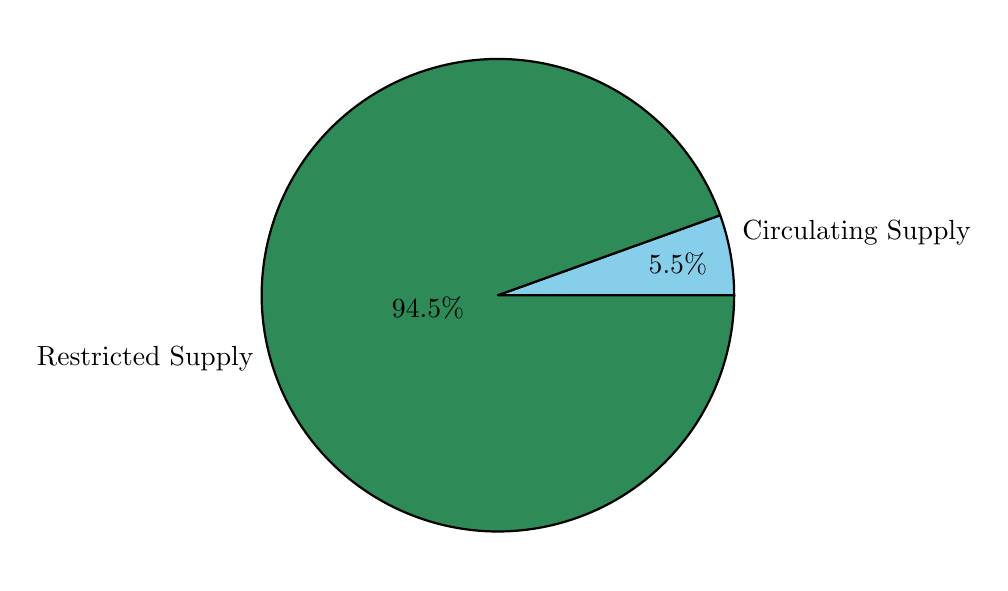
\begin{tikzpicture}
    \pie[color={SkyBlue, SeaGreen}] {5.5/Circulating Supply, 94.5/Restricted Supply}
\end{tikzpicture}
\captionof{figure}{\$JKL Launch Circulation}
\end{center}

\newcolumntype{C}{>{\centering\let\newline\\\arraybackslash\hspace{0pt}}m{2cm}}
\newcolumntype{f}{>{\columncolor{SkyBlue!50}}C}
\newcolumntype{g}{>{\columncolor{Gray!10}}C}

\newpage 
\section{Token Distributions}
\footnotetext[1]{As time comes closer to provide liquidity on various decentralized exchanges the community will be notified as to which exchanges will be used and how much they are incentivized.}

\small{
\hspace*{-2.5cm}
\begin{tabular}{| f | C | g | C | g | C | g | C |} 
\hline
\rowcolor{Black!80}
\color{White}Group & \color{White}Launch Ciruclation & \color{White}Vesting Total & \color{White}Year 1 Total Vested & \color{White}Year 2 Total Vested & \color{White}Year 3 Total Vested & \color{White}Year 4 Total Vested & \color{White}Launch Allocation \\
\hline
\hline
\cellcolor{Goldenrod!60} Development Entity & 24,900,000 & 24,900,000 & 6,225,000 & 12,450,000 & 18,675,000 & 24,900,000 & 24.9\% \\
\hline
\cellcolor{Goldenrod!60}Core Employees \& Contractors & 4,100,000 & 4,100,000 & 1,025,000 & 2,050,000 &  3,075,000 &  4,100,000  & 4.1\% \\
\hline
\cellcolor{YellowGreen!40}Pre-Seed Funding & 1,000,000 & 1,000,000 & 500,000 & 1,000,000 &  &  & 1\% \\
\hline
\cellcolor{YellowGreen!40}Seed Funding & 7,500,000, & 7,500,000, & 3,750,000 & 7,500,000 &  &  & 7.5\% \\
\hline
\cellcolor{Goldenrod!60}Advisors & 2,000,000 & 2,000,000 & 500,000 & 500,000 &500,000&500,000 & 2\% \\
\hline
Airdrop & 5,000,000 &  &  &  &  &  & 1.67\% \\
\hline
Dex Liquidity & 500,000\footnotemark[1] &  &  &  &  &  & 0.5\% \\
\hline
Launch Expenses \& Incentivized Testing & 500,000 &  &  &  &  &  & 0.5\% \\
\hline
Grants and Bounties  & 17,000,000 & 17,000,000 & 5,666,666.67 & 11,333,333.33 & 17,000,000 &  & 17\% \\
\hline
LP Rewards  & 15,000,000 &  &  &  &  &  & 15\% \\
\hline
\cellcolor{YellowGreen!40}Fundraising Remainder & 10,000,000 &  &  &  &  &  & 10\% \\
\hline
Community Pool & 12,500,000 & 12,500,000 & 4,166,666.67 & 8,333,333.33 & 12,500,000 &  & 12.5\% \\
\hline
\rowcolor{Goldenrod!60}
Total & 100,000,000 & 69,000,000 &  &  &  &  & 100\% \\
\hline
\end{tabular}
}
\captionof{table}{Token Distributions}


\newpage
\section{The Airdrop}
The triple snapshot to Juno Network, Cosmos Hub, and Secret Network stakers was completed on 4/9/2022 at 1pm EST and took around 24 hours to come to download all the data. 
The following algorithm and data were used to airdrop amounts for these stakers:

\begin{center}
\begin{tabular}{| l | l |}
\hline
\rowcolor{Black!80}
\color{White}Chain & \color{White}Eligible Wallets \\
\hline
\hline
Secret & 25,694 \\
\hline
\rowcolor{Black!5}
Juno & 79,473 \\
\hline
Atom & 190,337 \\ 
\hline
\rowcolor{Goldenrod!60}
Total & 295,504 \\
\hline
\end{tabular}
\captionof{table}{Airdrop Chain Spread}
\end{center}

\subsection{Airdrop Formula}

The airdrop formula is a clustered stepwise logarithmic function with lower and upper boundaries. We’ll
break this down.
\begin{itemize}
\item Clustered-This means that each chain is broken down into subgroups (or clusters) of tokens by the
amount staked. For example, the minimum amount staked is its own cluster.
\item Stepwise-This means that clusters are not continuous. So, moving from one cluster to another means
that there is an incremental number of tokens moving from one cluster to another.
\item Logarithmic- This function ensures an asymptotic cap when nearing the top of a certain cluster.
\item Lower and upper boundaries- this simply means that there is a minimum amount staked needed to
receive the airdrop as well as a whale cap.
\end{itemize}
The following tables can be used to calculate the approximate amount of \$JKL received when the
corresponding staked amount of each token.

\subsubsection{Secret Network Chain}
\begin{center}
\begin{tabular}{|c|c|}
\hline
\rowcolor{Black!80}
\color{White}Amount of \$SCRT Staked & \color{White}Approximate Amount of \$JKL Received \\
\hline
\hline
$20$ (minimum) & $0.74$ \\
\hline
\rowcolor{Black!10}
$20<x<100$ & ${(x+\frac{\log x}{2})*\frac{1666666*0.0015}{65153}}$ \\
\hline
$100<x<999.9$ & ${(x+\frac{\log x}{2})*\frac{1666666*0.0016}{65153}}$ \\
\hline
\rowcolor{Black!10}
$999.9<x<9999.99$ & ${(x+\frac{\log x}{2})*\frac{1666666*0.0017}{65153}}$\\
\hline
$9999.99<x<24769$ & ${(x+\frac{\log x}{2})*\frac{1666666*0.0018}{65153}}$ \\
\hline
\rowcolor{Black!10}
$24769<x$ & $1221.34$ \\
\hline
\end{tabular}
\end{center}

\paragraph{Example:}

For example, if I have 50 \$SCRT Staked I can expect around ${(50+\frac{\log 50}{2})*\frac{1666666*0.0015}{65153}} \approx1.95$ \$JKL tokens. \footnote[2]{If you are staking on the Jackal Validator you can multiply the airdrop reward by 2.}

\subsubsection{Juno Network Chain}
\begin{center}
\begin{tabular}{|c|c|}
\hline
\rowcolor{Black!80}
\color{White}Amount of \$JUNO Staked & \color{White}Approximate Amount of \$JKL Received \\
\hline
\hline
$10$ (minimum) & $0.76$ \\
\hline
\rowcolor{Black!10}
$10<x<100$ & ${(x+\log x)*0.07}$ \\
\hline
$100<x<999.9$ & ${(x+\log x)*0.071}$ \\
\hline
\rowcolor{Black!10}
$999.9<x<9999.99$ & ${(x+\log x)*0.072}$ \\
\hline
$9999.99<x<29159.25$ & ${(x+\log x)*0.073}$ \\
\hline
\rowcolor{Black!10}
$29159.25<x$ & $2304.42$ \\
\hline
\end{tabular}
\end{center}

\paragraph{Example:}

For example, if I have 50 \$JUNO Staked I can expect around $(50+\log 50)*0.07\approx3.618$ \$JKL tokens. 

\subsubsection{Cosmos Network Chain}
\begin{center}
\begin{tabular}{|c|c|}
\hline
\rowcolor{Black!80}
\color{White}Amount of \$ATOM Staked & \color{White}Approximate Amount of \$JKL Received \\
\hline
\hline
$10$ (minimum) & $ 0.327$ \\
\hline
\rowcolor{Black!10}
$10<x<100$ & ${(x+\log x)*0.02979}$ \\
\hline
$100<x<999.9$ & ${(x+\log x)*0.03}$ \\
\hline
\rowcolor{Black!10}
$999.9<x<9999.99$ & ${(x+\log x)*0.0305}$ \\
\hline
$9999.99<x<29999.99$ & ${(x+\log x)*0.0307}$ \\
\hline
\rowcolor{Black!10}
$30000<x$ & $973.54$ \\
\hline
\end{tabular}
\end{center}

\paragraph{Example:}

For example, if I have 50 \$ATOM Staked I can expect around $(50+\log 50)*0.02979\approx1.54$ \$JKL tokens. 

\section{Governance}
Jackal Protocol will be an L1 blockchain on the Cosmos IBC and will be subject to governance by the holders of
\$JKL as well as follow the typical Cosmos SDK governing model. The cost of making a proposal will be 1000
\$JKL. There are 5 different types of proposals.
In accordance with the Cosmos SDK \verb|gov| module as described in the \href{https://v1.cosmos.network/resources/whitepaper}{Cosmos Whitepaper}, governance is
done on-chain. Holders of the tokens can vote on proposals with a 1:1 bias, this means that if I have 10 \$JKL,
my vote is worth ½ the vote of someone who is holding 20 \$JKL. Anyone can submit proposals, these
proposals can be defined into 5 types.

\begin{itemize}
\item \textbf{Text Proposal:} A simple proposal that does not alter any source code such as opinion polls.
\item \textbf{Software Upgrade Proposal:} Validators update their software according to the specifications laid out in the
proposal.
\item \textbf{Community Pool Spend Proposal:} If accepted, the proposed amount enters the proposer’s wallet.
\item \textbf{Parameter Change Proposal:} Parameters of the network are changed such as the max validator count.
\item \textbf{Cancel Software Upgrade Proposal:} A vote to cancel any software update in the event that there is an
update set to release that wasn’t proposed in the community governance.

\end{itemize}

\subsection{Validators \& Delegations}
During the voting period, any \$JLK holder is permitted to vote on a proposal with their current holding amount
as the voting weight. If a holder chooses not to vote, all of the \$JKL they have delegated is under the control of
the validators they are delegating to.
For example, if I have 20 \$JKL delegated to ValidatorA, and 50 \$JKL delegated to ValidatorB, ValidatorA can
vote with my 20 \$JKL weight, as such ValidatorB can vote with my 50 \$JKL unless I vote on the proposal
myself. In the case I choose to vote, the combined 70 \$JKL is used to vote on whatever my personal choice
was and the 70 \$JKL is removed from their voting power for that particular proposal.

\section{Revenue Distribution}
The \$JKL token is a value accrual token for all decentralized applicatons on the Protocol. Once revenue is generated, \$JKL
tokens are either burned, redistributed, or a combination of both relivant to the economic relevant needs of the
protocol.

\subsection{Genesis Liquidity}
Upon genesis there will be liquidity provided on the Osmosis decentralized exchange to begin trading and arbitrage.
Initially there will be two pools each consisting of a \$JKL trading pair and \$ATOM and \$OSMO
respectively.  

\subsection{The Jackal Swap}
ackal Protocol will include an automated market maker (AMM) which provides three functions.  The primary goal of this AMM
is to avoid the use of a price oracle as we believe that arbitrage methods of the tokens that 
provided on the AMM will have a more accurate price locally on the AMM as well as globally 
across the market with fewer security flaws.  The secondary goal is to provide ease
of user experience on the Jackal platform so that users can swap between assets from the dashboard and wallet. 
The third fuction is to provide arbitrage opportunities above and beyond the use of initial price matching 
so that users have the potential to swap and earn rewards on this platform.  

\newpage
\begin{center}
\begin{figure}
\centering
\hspace*{-2.5cm}
\includegraphics[width=1.3\textwidth]{chart3.png}
\caption{Reveune Distribution}
\end{figure}
\end{center}


\newpage
\begin{thebibliography}{9}
\bibitem{website}
PancakeSwap. \emph{PancakeSwap Emission Rate.}

\url{https://docs.pancakeswap.finance/tokenomics/cake/cake-tokenomics}

\bibitem{website}
Helium. \emph{The Helium Consensus Protocol.}

\url{https://docs.helium.com/blockchain/consensus-protocol}

\bibitem{website}
Apollo Protocol. \emph{Apollo Tokenomics.}

\url{https://www.loop.markets/apollo-tokenomics-article/}

\bibitem{website}
Badger Protocol. \emph{Badger.}

\url{https://badger.com/products/badger}

\bibitem{website}
Pylon Protocol. \emph{Introducing Pylon Protocol.}

\url{https://medium.com/terra-money/pylon-protocol-e2a622ac553e}


\bibitem{website}
Terra Protocol. \emph{How the Terra Protocol Works.}

\url{https://docs.terra.money/docs/learn/protocol.html}

\bibitem{website}
Secret Network. \emph{Gray Paper.}

\url{https://scrt.network/graypaper}

\bibitem{website}
Shade Protocol. \emph{An Array of Connected Privacy-Preserving DeFi Applications.}

\url{https://shadeprotocol.io/pdf/Shade_Protocol_Whitepaper.pdf}

\bibitem{website}
Filecoin. \emph{Engineering Filecoin’s Economy.}

\url{https://filecoin.io/2020-engineering-filecoins-economy-en.pdf}

\bibitem{website}
Cosmos. \emph{Cosmos Whitepaper.}

\url{https://v1.cosmos.network/resources/whitepaper}

\end{thebibliography}




\newpage
\section{Disclaimers}
\tiny{
\textbf{Token Documentation:} Nothing in this document or the Website constitutes any offer by the Company, the Distributor, or the JACKAL team to sell any JKL (as defined
herein) nor shall it or any part of it nor the fact of its presentation form the basis of or be relied upon in connection with, any contract or investment decision. Nothing contained
in this document or the Website is or may be relied upon as a promise, representation or undertaking as to the future performance of JACKAL. The agreement between the
Distributor (or any third party) and you, in relation to any distribution or transfer of JKL, is to be governed only by the separate terms and conditions of such agreement. The
information set out in this document and the Website is for community discussion only and is not legally binding. No person is bound to enter into any contract or binding legal
commitment in relation to the acquisition of JKL, and no digital asset or other form of payment is to be accepted on the basis of this document or the Website. The agreement
for distribution of JKL and/or continued holding of JKL shall be governed by a separate set of Terms and Conditions or Token Distribution Agreement (as the case may be)
setting out the terms of such distribution and/or continued holding of JKL (the Terms and Conditions), which shall be separately provided to you or made available on the
Website. The Terms and Conditions must be read together with this document. In the event of any inconsistencies between the Terms and Conditions and this document or
the Website, the Terms and Conditions shall prevail.
\newline\newline
\textbf{Deemed Representations and Warranties:} By accessing this document or the Website (or any part thereof), you shall be deemed to represent and warrant to the Company,
the Distributor, their respective affiliates, and the JACKAL team as follows:\newline\newline
(a) in any decision to acquire any JKL, you have shall not rely on any statement set out in this document or the Website;\newline\newline
(b) you will and shall at your own expense ensure compliance with all laws, regulatory requirements and restrictions applicable to you (as the case may be);\newline\newline
(c) you acknowledge, understand and agree that JKL may have no value, there is no guarantee or representation of value or liquidity for JKL, and JKL is not an investment
product nor is it intended for any speculative investment whatsoever;\newline\newline
(d) none of the Company, the Distributor, their respective affiliates, and/or the JACKAL team members shall be responsible for or liable for the value of JKL, the transferability
and/or liquidity of JKL and/or the availability of any market for JKL through third parties or otherwise; and \newline\newline
(e) you acknowledge, understand and agree that you are not eligible to participate in the distribution of JKL if you are a citizen, national, resident (tax or otherwise), domiciliary
and/or green card holder of a geographic area or country (i) where it is likely that the distribution of JKL would be construed as the sale of a security (howsoever named),
financial service or investment product and/or (ii) where participation in token distributions is prohibited by applicable law, decree, regulation, treaty, or administrative act
(including without limitation the United States of America and the People's Republic of China); and to this effect, you agree to provide all such identity verification document
when requested in order for the relevant checks to be carried out.\newline\newline

The Company, the Distributor and the JACKAL team do not and do not purport to make, and hereby disclaims, all representations, warranties or undertaking to any entity or
person (including without limitation warranties as to the accuracy, completeness, timeliness, or reliability of the contents of this document or the Website, or any other
materials published by the Company or the Distributor). To the maximum extent permitted by law, the Company, the Distributor, their respective affiliates and service providers
shall not be liable for any indirect, special, incidental, consequential or other losses of any kind, in tort, contract or otherwise (including, without limitation, any liability arising
from default or negligence on the part of any of them, or any loss of revenue, income or profits, and loss of use or data) arising from the use of this document or the Website,
or any other materials published, or its contents (including without limitation any errors or omissions) or otherwise arising in connection with the same. Prospective acquirors of
JKL should carefully consider and evaluate all risks and uncertainties (including financial and legal risks and uncertainties) associated with the distribution of JKL, the
Company, the Distributor and the JACKAL team.\newline\newline

\textbf{JKL Token:} JKL is designed to be utilized, and that is the goal of the JKL distribution. In fact, the project to develop JACKAL would fail if all JKL holders simply held onto their
JKL and did nothing with it. In particular, it is highlighted that JKL:\newline\newline
(a) does not have any tangible or physical manifestation, and does not have any intrinsic value(nor does any person make any representation or give any commitment as to its
value);\newline\newline
(b) is non-refundable and cannot be exchanged for cash (or its equivalent value in any other digital asset) or any payment obligation by the Company, the Distributor or any of
their respective affiliates;\newline\newline
(c) does not represent or confer on the token holder any right of any form with respect to the Company, the Distributor (or any of their respective affiliates), or its revenues or
assets, including without limitation any right to receive future dividends, revenue, shares, ownership right or stake, share or security, any voting, distribution, redemption,
liquidation, proprietary (including all forms of intellectual property or licence rights), right to receive accounts, financial statements or other financial data, the right to requisition
or participate in shareholder meetings, the right to nominate a director, or other financial or legal rights or equivalent rights, or intellectual property rights or any other form of
participation in or relating to JACKAL, the Company, the Distributor and/or their service providers;\newline\newline
(d) is not intended to represent any rights under a contract for differences or under any other contract the purpose or pretended purpose of which is to secure a profit or avoid
a loss;\newline\newline
(e) is not intended to be a representation of money (including electronic money), security, commodity, bond, debt instrument, unit in a collective investment scheme or any
other kind of financial instrument or investment;\newline\newline
(f) is not a loan to the Company, the Distributor or any of their respective affiliates, is not intended to represent a debt owed by the Company, the Distributor or any of their
respective affiliates, and there is no expectation of profit; and\newline\newline
(g) does not provide the token holder with any ownership or other interest in the Company, the Distributor or any of their respective affiliates. Notwithstanding the JKL
distribution, users have no economic or legal right over or beneficial interest in the assets of the Company, the Distributor, or any of their affiliates after the token distribution.\newline\newline
To the extent, a secondary market or exchange for trading JKL does develop, it would be run and operated wholly independently of the Company, the Distributor, the
distribution of JKL and JACKAL. Neither the Company nor the Distributor will create such secondary markets nor will either entity act as an exchange for JKL.\newline

\textbf{Informational purposes only:} The information set out herein is only conceptual, and describes the future development goals for JACKAL to be developed without any binding
commitment. Please do not rely on this information in deciding whether to participate in the token distribution because ultimately, the development, release, and timing of any
products, features or functionality remains at the sole discretion of the Company, the Distributor or their respective affiliates, and is subject to change. Further, this document
or the Website may be amended or replaced from time to time. There are no obligations to update this document or the Website, or to provide recipients with access to any
information beyond what is provided herein.\newline

\textbf{Regulatory approval:} No regulatory authority has examined or approved, whether formally or informally, any of the information set out in this document or the Website. No
such action or assurance has been or will be taken under the laws, regulatory requirements or rules of any jurisdiction. The publication, distribution or dissemination of this
document or the Website does not imply that the applicable laws, regulatory requirements or rules have been complied with.\newline

\textbf{Cautionary Note on forward-looking statements:} All statements contained herein, statements made in press releases or in any place accessible by the public and oral
statements that may be made by the Company, the Distributor and/or the JACKAL team, may constitute forward-looking statements (including statements regarding the intent,
belief or current expectations with respect to market conditions, business strategy and plans, financial condition, specific provisions and risk management practices). You are
cautioned not to place undue reliance on these forward-looking statements given that these statements involve known and unknown risks, uncertainties and other factors that
may cause the actual future results to be materially different from that described by such forward-looking statements, and no independent third party has reviewed the
reasonableness of any such statements or assumptions. These forward-looking statements are applicable only as of the date indicated in this document, and the Company,
the Distributor, as well as the JACKAL team, expressly disclaim any responsibility (whether express or implied) to release any revisions to these forward-looking statements to
reflect events after such date.\newline

\textbf{References to companies and platforms:} The use of any company and/or platform names or trademarks herein (save for those which relate to the Company, the Distributor
or their respective affiliates) does not imply any affiliation with, or endorsement by, any third party. References in this document or the Website to specific companies and
platforms are for illustrative purposes only.\newline

\textbf{English language:} This document and the Website may be translated into a language other than English for reference purposes only and in the event of conflict or ambiguity
between the English language version and translated versions of this document or the Website, the English language versions shall prevail. You acknowledge that you have
read and understood the English language version of this document and the Website.\newline

\textbf{No Distribution:} No part of this document or the Website is to be copied, reproduced, distributed or disseminated in any way without the prior written consent of the Company
or the Distributor. By attending any presentation on this document or by accepting any hard or soft copy of this document, you agree to be bound by the foregoing limitations.
}


\newpage

\section{Changelog}

\normalsize
\begin{itemize}
\item Changed: Reformatted forumlas in airdrop calculation tables.
\item Added: Examples of calculations in airdrop tables.
\item Added: Changelog.
\item Fixed: Typos.
\item Fixed: Made document easy on the eyes.
\item Changed: Instances of the word DAO and changed them to Protocol
\item Added: Infomration about the AMM
\item Changed: General information about the tokenomics

\end{itemize}



\end{document}

